% GENERATED by scripts/make_figures.py from report/data/report_data.json. Do not edit; regenerate.
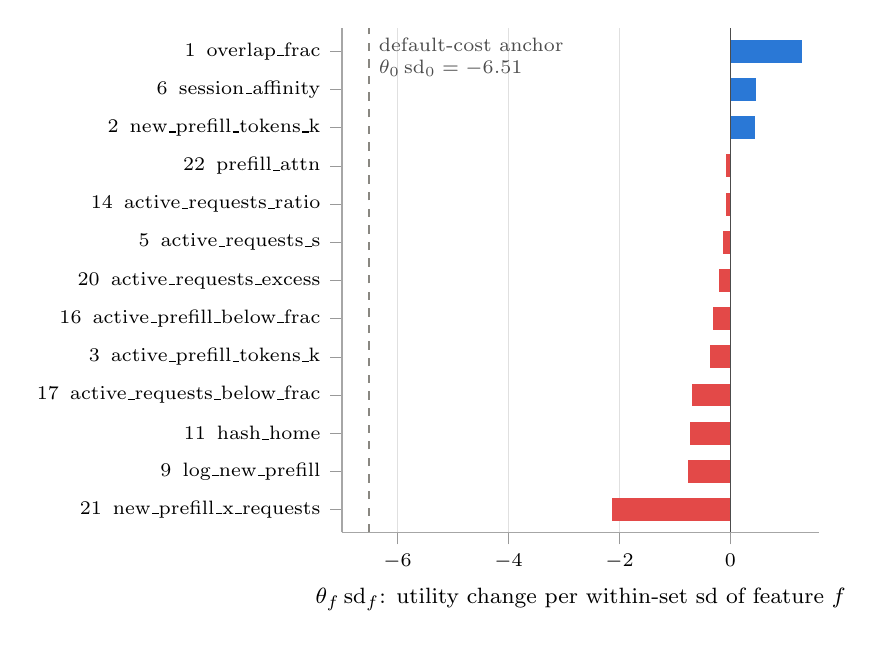
\begin{tikzpicture}
\begin{axis}[
  width=0.5\linewidth, height=6.4cm,
  scale only axis,
  tick label style={font=\scriptsize}, label style={font=\footnotesize, align=center},
  scaled ticks=false, tick label style={/pgf/number format/fixed},
  tick align=outside, tick style={black!40}, axis line style={black!35},
  axis x line*=bottom, axis y line*=left,
  grid style={black!12, line width=0.4pt},
  legend style={font=\scriptsize, draw=none, fill=white, fill opacity=0.85, text opacity=1},
  legend cell align=left,
  ymin=-0.6, ymax=12.6, ytick={0,1,2,3,4,5,6,7,8,9,10,11,12},
  yticklabels={{21\enspace\code{new\_prefill\_x\_requests}},{9\enspace\code{log\_new\_prefill}},{11\enspace\code{hash\_home}},{17\enspace\code{active\_requests\_below\_frac}},{3\enspace\code{active\_prefill\_tokens\_k}},{16\enspace\code{active\_prefill\_below\_frac}},{20\enspace\code{active\_requests\_excess}},{5\enspace\code{active\_requests\_s}},{14\enspace\code{active\_requests\_ratio}},{22\enspace\code{prefill\_attn}},{2\enspace\code{new\_prefill\_tokens\_k}},{6\enspace\code{session\_affinity}},{1\enspace\code{overlap\_frac}}},
  xmin=-7, xmax=1.6, xmajorgrids,
  xlabel={$\theta_f\,\mathrm{sd}_f$: utility change per within-set sd of feature $f$},
  clip=false,
]
% data: coef.21
\addplot[xbar, bar shift=0pt, bar width=0.6, fill={rgb,255:red,227;green,73;blue,72}, draw=none, forget plot] coordinates {(-2.128489075926415,0.0)};
% data: coef.9
\addplot[xbar, bar shift=0pt, bar width=0.6, fill={rgb,255:red,227;green,73;blue,72}, draw=none, forget plot] coordinates {(-0.7623893316636174,1.0)};
% data: coef.11
\addplot[xbar, bar shift=0pt, bar width=0.6, fill={rgb,255:red,227;green,73;blue,72}, draw=none, forget plot] coordinates {(-0.7383408125966545,2.0)};
% data: coef.17
\addplot[xbar, bar shift=0pt, bar width=0.6, fill={rgb,255:red,227;green,73;blue,72}, draw=none, forget plot] coordinates {(-0.6986997281194663,3.0)};
% data: coef.3
\addplot[xbar, bar shift=0pt, bar width=0.6, fill={rgb,255:red,227;green,73;blue,72}, draw=none, forget plot] coordinates {(-0.36126360489603904,4.0)};
% data: coef.16
\addplot[xbar, bar shift=0pt, bar width=0.6, fill={rgb,255:red,227;green,73;blue,72}, draw=none, forget plot] coordinates {(-0.31793560403582644,5.0)};
% data: coef.20
\addplot[xbar, bar shift=0pt, bar width=0.6, fill={rgb,255:red,227;green,73;blue,72}, draw=none, forget plot] coordinates {(-0.20242523761742345,6.0)};
% data: coef.5
\addplot[xbar, bar shift=0pt, bar width=0.6, fill={rgb,255:red,227;green,73;blue,72}, draw=none, forget plot] coordinates {(-0.1287358962783343,7.0)};
% data: coef.14
\addplot[xbar, bar shift=0pt, bar width=0.6, fill={rgb,255:red,227;green,73;blue,72}, draw=none, forget plot] coordinates {(-0.08966912381406741,8.0)};
% data: coef.22
\addplot[xbar, bar shift=0pt, bar width=0.6, fill={rgb,255:red,227;green,73;blue,72}, draw=none, forget plot] coordinates {(-0.08446106952593102,9.0)};
% data: coef.2
\addplot[xbar, bar shift=0pt, bar width=0.6, fill={rgb,255:red,42;green,120;blue,214}, draw=none, forget plot] coordinates {(0.44851952512983045,10.0)};
% data: coef.6
\addplot[xbar, bar shift=0pt, bar width=0.6, fill={rgb,255:red,42;green,120;blue,214}, draw=none, forget plot] coordinates {(0.4513385789422368,11.0)};
% data: coef.1
\addplot[xbar, bar shift=0pt, bar width=0.6, fill={rgb,255:red,42;green,120;blue,214}, draw=none, forget plot] coordinates {(1.289157937216578,12.0)};
% data: anchor
\addplot[color={rgb,255:red,137;green,135;blue,129}, dashed, line width=0.6pt, no marks, forget plot] coordinates {(-6.5099599822061185,-0.6) (-6.5099599822061185,12.6)};
\node[anchor=north west, font=\scriptsize, text=black!70, align=left] at (axis cs:-6.5099599822061185,12.6) {default-cost anchor\\$\theta_0\,\mathrm{sd}_0 = -6.51$};
\draw[black!70, line width=0.6pt] ({axis cs:0.0,0} |- {rel axis cs:0,0}) -- ({axis cs:0.0,0} |- {rel axis cs:0,1});
\end{axis}
\end{tikzpicture}
